\documentclass[11pt]{article}

\usepackage[utf8]{inputenc}
\usepackage{acl2015}
%\usepackage{url}
\usepackage{natbib}
\usepackage{graphicx}
\usepackage{multicol}
\usepackage{hyperref}
\usepackage{threeparttable}
\usepackage{algorithm2e}

\title{This Time With Feeling: Sentiment to ML Headlines}

\author{Ben Arnoldy \\
  University of California, Berkeley \\
  {\tt arnoldyb@berkeley.edu} \\\And
  Mark Paluta \\
  University of California, Berkeley \\
  {\tt mpaluta@berkeley.edu} \\}
  
\date{July 2019}

\begin{document}

\maketitle

\begin{abstract}
    
\end{abstract}

\section{Introduction}
The art of good headline writing is not as simple as summarizing relevant details; it requires wit, originality, and a tone that matches the piece. Algorithms have made improvements in summarization, but still struggle with these more nuanced elements. Despite this shortcoming, algorithms could still be useful to an editor, suggesting a number of possible headlines to provide inspiration or for the editor to refine and synthesize into a final product. We propose an incremental improvement in automatic headline generation by incorporating tonal bias to match the underlying content.

\section{Background}
Headline generation is primarily approached as a single-document summarization task. The nature of headlines makes them relatively more difficult to produce with machine learning than typical document summaries. First, headlines tend to be shorter than the average sentence, requiring greater concision than typical ML summaries of one or more sentences. Additionally, they are often written in a short-hand style different from the body text, making extractive summarization theoretically less suitable than the more challenging task of abstractive summarization. 

Current methods of summarization involve an encoder-decoder architecture \citep{rush2015neural} with a ROUGE evaluation metric \cite{Ayana2017}. ROUGE is a recall-oriented metric to score a generated summary against a reference summary \cite{lin-2004-rouge}. Specific variants include ROUGE-N, scoring the number of common N-grams, and ROUGE-L, scoring the longest common subsequence. Recent refinements to headline generation include adversarial reward systems to combat repetition \cite{DBLP:journals/corr/abs-1902-07110} and applying state-of-the-art Transformer algorithms \cite{DBLP:journals/corr/abs-1901-07786}.

While most work on headline generation focuses exclusively on summarization, two recent papers in other summarization domains explored efforts to add desired sentiment. One naive approach from Chaudhari et al \cite{DBLP:journals/corr/abs-1802-09426} pre-processed sentences in the body of the corpus to generate sentence-level sentiment scores that characterize the emotional tone of the text. Sentences that did not match the desired sentiment polarity (positive or negative) were dropped before training the summarization model. Another more elaborate approach from Hu et al \cite{DBLP:journals/corr/HuYLSX17} to produce customer review summaries added a discriminator to evaluate the sentiment of generated summaries, looping back to the generator to optimize on this additional criterion. 

\section{Methodology}

\subsection{Objective}
We build a Universal Transformer architecture, basing our algorithm off of that of Gavrilov et al \cite{DBLP:journals/corr/abs-1901-07786}, but adding sentiment into the model in the spirit of Chaudhari   \cite{DBLP:journals/corr/abs-1802-09426} and Hu \cite{DBLP:journals/corr/HuYLSX17}. We use sentiment-based preprocessing to upsample examples where sentiment matches well between body and headline and downsample those where the match is poor. Our objective is to increase the sentiment match between an article's headline and body while simultaneously obtaining similar ROUGE scores.

\subsection{Workflow}

The workflow we defined to pre-process, train, and evaluate our data can be seen in algorithm \ref{alg:1}. Note that the algorithm can be parallelized across three virtual machines for the three filtering options.

Not married to this format, but getting the content in for now.

\begin{algorithm}[H]
\SetAlgoLined
 \For{filtering in (none, sentiment, random)}{
    1: pre-processing and metadata generation\;
    2: randomize train-dev-test split\;
    3: \If{filtering = sentiment}{
        4: sentiment-based downsampling\;}
    5: \If{filtering = sentiment}{
        6: random downsampling\;}
    7: train on training set\;
    8: decode dev or test set\;
    9: score ROUGE metrics
    10: score sentiment metric\;
 }
 \caption{End-to-end pipeline}
\label{alg:1}
\end{algorithm}

\subsection{Universal Transformer Architecture}
We use an encoder-decoder architecture, AdamW optimizer, and the set of specific hyperparameters outlined by Gavrilov et al \cite{DBLP:journals/corr/abs-1901-07786} as our baseline. Noteworthy parameters are listed in Table \ref{table:1}. A diagram of the architecture can be viewed in Figure \ref{figure:1}.

\begin{table}[h!]
\centering
\begin{tabular}{|c | c|} 
 \hline
 Hyperparameter & Value \\ [0.5ex] 
 \hline
 Hidden layer size & 1024 \\ 
 Filter size & 4096 \\
 Heads of attention & 8 \\
 Layer preprocess sequence & None \\
 Layer postprocess sequence & dropout \\
 & $\rightarrow$ add $\rightarrow$ \\
 & normalize \\
 Postprocess dropout & 0.3 \\
 Encoder layers & 4 \\
 Decoder layers & 4 \\
 Learning rate warmup steps & 4000 \\ [1ex]
 \hline
\end{tabular}
\caption{Noteworthy Hyperparameters}
\label{table:1}
\end{table}

\begin{figure}[h!]
\centering
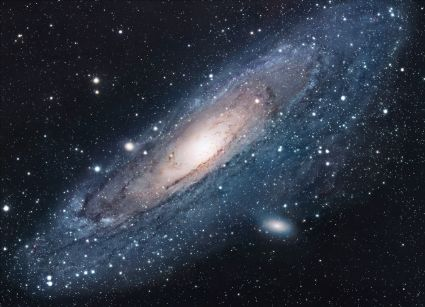
\includegraphics[scale=1.7]{universe}
\caption{Universal Transformer Architecture}
\label{figure:1}
\end{figure}

\subsection{corpus}
We use the \href{https://catalog.ldc.upenn.edu/LDC2008T19}{New York Times annotated corpus} to match Gavrilov. This contains 1.8 million New York Times articles spanning from 1987 to 2007. Like Gavrilov, we filtered out obituaries and articles with wordcount < XX or > 2000 and headline length < 3 or > XX. We were left with XXXXXX articles, which we then split along 70:10:20 proportions into train, dev, and test datasets.

\subsection{Sentiment analysis}
We use a positive-negative polarity function as most research on sentiment is a simple positive-negative scale and we wish to leverage existing work. Following [racist AIXXXX's model, we take Bing Liu's opinion lexicon [XXX] -- a list of around 6,800 words that are labeled either positive or negative -- and embed the lexicon's words in pre-trained GloVe embeddings. These embeddings and their [0,1] labels are used to train a logistic regression model that returns the log probability of a new word being positive and the log probability of it being negative. The negative probability is subtracted from the positive to arrive at a score; positive scores indicate positive associations and vice versa. To score an entire headline, we sum the individual scores of all the words in the headline and take an average. We construct a filter to remove articles where the polarity of the headline and its short summary (i.e. lede) differ, as shown in figure XXX (write it as an xor).

\subsection{Evaluation}
To test the quality of generated headlines, we employ the same variants on the ROUGE metric as Gavrilov et al for effective comparison of results.

Discuss post-decoder scoring of sentiment.

\subsection{Implementation}
Specifically, we chose to work with the package \href{https://github.com/tensorflow/tensor2tensor}{\texttt{tensor2tensor}}. This package was developed by the Google Brain team and is designed for furthering research on a variety of natural language processing problems. We began by replicating the CNN/Daily Mail text summarization problem. We then adapted the architecture to accommodate a new problem of summarization, specifically headline generation rather than key point summarization, on the New York Times annotated corpus. The specific adaptations we had to make were as follows:

\begin{itemize}
    \item Prepare New York Times corpus for \texttt{tensor2tensor} ingestion by extracting filepath, headline, body, lede, word count, and other metadata, writing this data to a lot file, and performing a random train/dev/test split
    \item Define problem \texttt{Gavrilov} inheriting \texttt{Text2TextProblem}
    \item Apply a subword tokenizer to imitate Gavrilov et al's BPE tokenization
    \item Override a variety of default Universal Transformer hyperparameters as defined in Table \ref{table:1}
    \item Create optional sentiment pre-processing step
    \item Create optional random down-sampling step for control
\end{itemize}

\section{Results}
\subsection{Decoder}

Unfortunately, the decoder 

Example

\begin{table}[h!]
\centering
\begin{tiny}
\begin{tabular}{|p{7cm}|} 
 \hline
 \textbf{Input:} When Democratic Rep. Rashida Tlaib accused Republican Rep. Mark Meadows of racism earlier this year, one of his "best friends," House Oversight Committee chairman and Democratic Rep. Elijah Cummings immediately jumped to his defense. When Cummings was attacked on similar grounds by President Donald Trump over the weekend, it took a bit longer for Meadows to publicly repay the favor. On Saturday and Sunday, Trump went after Cummings on Twitter, calling the veteran Democratic lawmaker a "racist" and his district a "disgusting, rat and rodent infested mess." Trump's comments hung in the air for days, sparking yet another conversation about the President's race-focused rhetoric. Republicans largely stayed silent, including Meadows, whose warm relationship with Cummings prompted questions about his reticence to defend his friend. \\ [0.5ex] 
 \hline
 \textbf{Output:} Fatah Fatah Fatah Fatah Mitch Mitch Mitch Mitch Mitch Mitch Mitch Mitch Mitch Mitch Mitch Mitch Mitch Mitch Mitch Mitch Mitch Mitch Mitch Mitch Mitch Mitch Boys Boys Boys Boys Boys Boys Boys Boys Boys Boys Boys Fatah Fatah Fatah Fatah Fatah Boys Boys Boys Boys Boys Mitch Mitch Boys Boys Boys Mitch Mitch Mitch Fatah Fatah Fatah Boys Boys Mitch Mitch Mitch Mitch Mitch Mitch Boys Boys Boys Fatah Fatah Fatah Mitch Mitch Mitch Mitch Mitch Mitch Fatah Fatah Fatah Mitch Mitch Mitch Mitch Mitch Mitch Boys Boys Mitch Mitch Mitch Mitch Mitch Mitch Boys Boys Boys Boys Boys Boys Boys Boys Boys Boys Boys Boys Boys Boys Mitch Mitch Boys Boys Boys Boys Boys Mitch Mitch Boys Boys Fatah god god god god god god god god god god god Mitch Mitch Mitch god Mitch Mitch Mitch Mitch Mitch Mitch Mitch Mitch Mitch Mitch Mitch Mitch Mitch Mitch Mitch Mitch Mitch Mitch Mitch Mitch Mitch Mitch Mitch Mitch Mitch Mitch Mitch Mitch Mitch Mitch Mitch Mitch Mitch Mitch Mitch Mitch Mitch Mitch Mitch Mitch Mitch Mitch Mitch Mitch Mitch Mitch Mitch  \\ 
 \hline
\end{tabular}
\end{tiny}
\caption{Example Output}
\label{table:3}
\end{table}

\subsection{ROUGE and sentiment scores}

insert table for ROUGE

Commentary about how we can't evalute sentiment due to decoder

\subsection{Resource considerations}

As we ran our algorithm on several different resource configurations, we decided to take the opportunity to record approximate computation times on various configurations to inform future resource requirements for future work, as some results were nonintuitive. Our approximate benchmarks can be seen in Table \ref{table:2}

\begin{table}[h!]
\begin{threeparttable}
\centering
\begin{tabular}{|p{2cm}|p{2.2cm}|p{2cm}|} 
 \hline
 Task & Configuration & Approx. Computation Time \\ [0.5ex] 
 \hline\hline
 Vocab Generation & CPU-heavy^{1} & 5 hr 40 min \\ 
 Vocab Generation & Balanced^{2} & 40 min \\
 \hline
 One training step & CPU-heavy & 3.9 sec \\
 One training step & Balanced & 9.7 sec \\ 
 One training step & GPU-heavy^{3} & I can do quick test for this later \\[1ex]
 \hline
\end{tabular}
\begin{tablenotes}\footnotesize
\item[1] 32 vCPUs on Google Cloud
\item[2] Nvidia 1060 GPU and Ryzen 7 2700 (8 cores, 16 threads)
\item[3] 8 vCPUs and Nvidia Tesla K80 on Google Cloud
\end{tablenotes}
\caption{Computational Benchmarks}
\end{threeparttable}
\label{table:2}
\end{table}

Of particular note, we observed that vocabulary generation was a GPU-intensive task and benefited greatly from the addition of a GPU. On the other hand, training was CPU-bottlenecked and even a competitive GPU with 8 vCPUs was outperformed by just 16 vCPUs with no GPU. This result in particular was surprising and led us to perform most of our intensive training on CPU-heavy configurations. It is also worth noting that the two configurations are of approximately equal cost given current Google Cloud pricing.

\section{Discussion}
\section{Conclusion}



\section{Materials}
Our materials for this project can be found at the following link:
\url{https://github.com/mpaluta/headline_generation}.

"citing Rush here" \citep{rush2015neural}
"citing Ayana here" \cite{Ayana2017}
"citing Peng Xu here" \cite{DBLP:journals/corr/abs-1902-07110}
"citing Gavrilov here" \cite{DBLP:journals/corr/abs-1901-07786}
"citing Chaudari here" \cite{DBLP:journals/corr/abs-1802-09426}
"citing Zhiting Hu here" \cite{DBLP:journals/corr/HuYLSX17}
"citing Lin here" \cite{lin-2004-rouge}
"citing Attention is all you Need here" \cite{DBLP:journals/corr/VaswaniSPUJGKP17}

\bibliographystyle{plain}
\bibliography{references}
\end{document}




